%Abstract - small description of the paper
\begin{abstract}
Steganography is the combination between the 2 Greek words : steganós (which means concealed) and graphia(which means writing) \cite{steganography-origin} and has been a method that humanity has used to hide information for more than 2 millenniums \cite{steganography-history}.
This paper presents both existing and new ways of embedding computer files and data into different digital multimedia formats as covert as possible and allowing the encoded information to be retrieved at a later time without any losses.
\end{abstract}

\section[Introduction to computer Steganography]{Introduction}

%\begin{figure}[H]
%    \centering
%    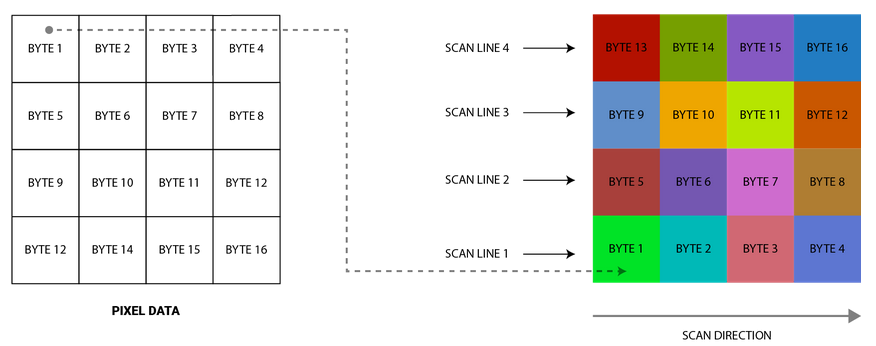
\includegraphics[]{pics/bmp_scan_line}
%    \caption{How BMP works}
%    \label{simulationfigure}
%\end{figure}

\begin{multicols}{2}

%introduction section
\subsection{Subsection Heading Here}
%subsection text
\end{multicols}


\begin{thebibliography}{9}
\bibitem{steganography-origin}
Merriam-Webster dictionary.
\\\texttt{https://www.merriam-webster.com/dictionary/steganography}

\bibitem{steganography-history}
Petitcolas FAP, Anderson RJ and Kuhn MG.
\textit{Information Hiding - A Survey}.
Proceedings of the IEEE, special issue on protection of multimedia content, 1999.
% http://www.creangel.com/papers/steganografia.pdf
\bibitem{seeing-the-unseen} 
Johnson Neil and Jajodia Susil.
\textit{Exploring Steganography : Seeing the Unseen}. 
Los Alamitos, IEEE Computer Society, 1998.

%http://www.academia.edu/download/54323461/EN_-_Image_Steganography_Overview.pdf
\bibitem{overview-image-steganography} 
T. Morkel, J.H.P. Eloff and M.S. Olivier. 
\textit{An overview of image steganography}.
University of Pretoria, ICSA Research Group, 2005.

%http://honeyman.org/u/provos/papers/practical.pdf
\bibitem{hide-and-seek} 
Niels Provos and Peter Honeyman.
\textit{Hide and Seek: An Introduction to Steganography}.
University of Michigan, IEEE Computer Society, 2003

\end{thebibliography}

